\chapter{Proof of concept d'une attaque}
\label{chap:attaque}

L'implémentation de \og \gls{safeStack} \fg au sein de \gls{llvm} doit permettre de prévenir les attaques se basant sur l'éxploitation d'un dépassement de tampon. Dans ce chapitre un \og proof of concept \fg d'une telle attaque est décrit sur un exemple de code fictif. Afin de rendre plus portable et reproductible cette phase de test, un environnement spécifique est mis en place et décrit précisément ainsi que la recette utilisée lors de la phase de compilation.

L'objectif est de démontrer l'efficacité de \gls{levee} et de comparer l'approche avec celle des \og \gls{stackCookies} \fg. Pour ce faire, une première attaque a été pensée, malheureusement celle-ci n'avais pas la possibilité d'aboutir. Basée sur ces conclusions, une autre attaque a été mise en place. Leur descriptions théorique ainsi que leurs implémentations sont décrites dans ce chapitre.

Un des exemples d'attaque proposé dans ce chapitre est basé sur l'article \og Introduction to return oriented programming (ROP) \fg du blog \textit{codearcana.com} \cite{IntroductionToROP}.

\minitoc

\newpage

% -----------------------------------------------------------------------------
\section{Environnement}

Afin de faciliter la mise en place de l'attaque, la compilation est faite en 32~bits. L'environnement choisi pour installer la version 4.0 de \gls{llvm} est Debian 8 en 64~bits. Afin de pouvoir correctement compiler et exécuter en 32~bits, les bibliothèques nécessaires doivent être installées (lignes 20 à 22). En plus de \gls{llvm}, \gls{gdb} ainsi que quelques autres utilitaires sont installés.

\subsection{Docker}

L'environnement décrit ci-dessus ainsi que l'installation des outils sont mis en place grâce à Docker. Le Dockerfile suivant contient toutes les instructions nécessaires afin d'installer la version 4.0 de \gls{llvm} et \gls{clang}.

\begin{listing}
	\dockerfile{02-main/listings/Dockerfile}
	\caption{Fichier décrivant l'environnement choisi pour l'installation de \gls{llvm} 4 sous Debian 8}
	\label{lst:dockerfile}
\end{listing}

Il existe plusieurs manières d'installer \gls{llvm}. Il serait tout à fait possible de compiler directement depuis les sources. Plusieurs de ces techniques ont été testées, et la suivante a été retenue: l'installation de Clang 4.0, \gls{lldb} (équivalant de \gls{gdb}) et de LLD (le \og linker \fg de \gls{llvm}) se fait en rajoutant le dépôt APT de \gls{llvm}. Après plusieurs essais, le débogueur \gls{gdb} est préféré à \gls{lldb} et est par la suite utilisé à la place de \gls{lldb}, ce dernier n'étant pas encore assez complet et globalement utilisé.

Tout les autres fichiers de configurations de l'environnement Docker sont disponibles à l'\autoref{chap:dockerConf}.

\subsection{Gestion de la compilation}

L'utilitaire \textit{make} est utilisé pour gérer le processus de compilation. Un Makefile est mis en place afin de rassembler les différents \og flags \fg utilisés pour générer les deux versions exécutables (l'un avec \gls{safeStack} et l'autre sans). En en-tête, différentes variables utilisées par \textit{make} sont définies afin de s'assurer que \gls{clang} 4.0 est bien utilisé. Deux version de l'exécutable sont créés: \textit{safe-stack} et \textit{stack-cookie}. Le language intermédiaire de \gls{llvm} est émis lors de la compilation afin de comparer les effets de l'un et l'autre mécanisme de protection.

À noter que la protection de la pile \texttt{\textit{-fstack-protector}} est desactivée grâce à \texttt{\textit{-fno-stack-protector}} lorsque l'on active \og \gls{safeStack} \fg. Le but étant de comparer les deux mécanismes, qui plus est, actuellement \og \gls{safeStack} \fg n'est pas compatible avec les \og \gls{stackCookies} \fg.

\begin{listing}
	\makefile{02-main/listings/Makefile}
	\caption{Makefile regroupant les différentes options de compilations}
	\label{lst:defaultMakefile}
\end{listing}

Un script permettant d'afficher les mécanismes de protection d'un binaire est utilisé, pour cela une règle spécifique aux tests est décrite à la ligne 38 du \autoref{lst:defaultMakefile}.

\vfill

\subsection{Mécanismes de sécurité actifs}

\gls{aslr} est actif au sein de l'environnement. Chaque binaire est protégé soit avec \og \gls{stackCookies} \fg ou avec \og \gls{safeStack} \fg. Le script \mintinline{bash}{checksec.sh} \cite{CheckSec} est utilisé pour afficher les mécanismes actifs sur chaque binaire. On peut constater sur le résultat ci-dessous que les \og \gls{stackCookies} \fg sont bien désactivés lors du test de \og \gls{safeStack} \fg et que dans les deux cas le drapeau \gls{nx} est actif.

\begin{listing}
	\textfile{02-main/listings/checksec.res}
	\caption{Resultat du test de sécurité par checksec.sh}
	\label{lst:checksecRes}
\end{listing}

\gls{pie} est un mécanisme de protection récent qui permet d'appliquer de l'aléatoire sur des régions de code, et ainsi rendre plus difficile la mise en place d'une attque de type \gls{rop}.


% -----------------------------------------------------------------------------
\section{Pointeur de fonction sur la pile}

\subsection{Description théorique de l'attaque}

La première tentative se base sur une \textit{structure} dans laquelle est stocké un pointeur vers une fonction. En plaçant la \textit{structure} et le tampon sur la pile d'exécution, l'idée est de réécrire l'adresse du pointeur présent dans ladite \textit{structure} afin de lancer la chaîne de gadgets à l'appel du pointeur.

Le but est de mettre en place une \og stack frame \fg correspondant à la fonction \mintinline{c}{main()} ayant les variables locales stockées dans l'ordre dans lesquelles elles sont déclarées, comme le montre la \autoref{fig:attackStructExpected}.

\begin{figure}[H]
	\centering
	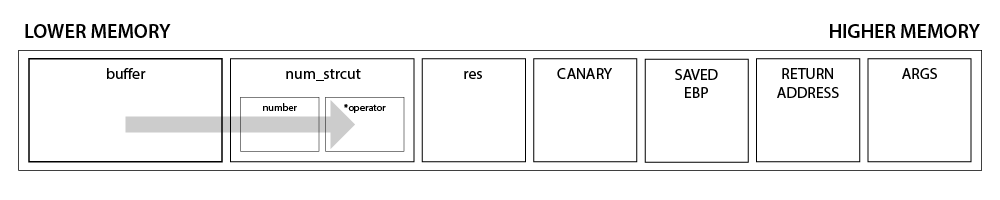
\includegraphics[width=1\columnwidth]{attackStructExpected}
	\captionsource{Résultat attendu de la \og stack frame \fg sur la première attaque}
	{Résultat attendu de la \og stack frame \fg sur la première attaque}
	{Auteur}
	\label{fig:attackStructExpected}
\end{figure}

\subsection{Implémentation}

Le code correspondant au scénario, présenté en \autoref{lst:struct}, comprend: (i) une structure nommée \texttt{Number}, (ii) une fonction \texttt{call()} permettant d'appliquer la fonction pointée par la structure et (iii) une fonction retournant le carré --- très mal optimisé --- de la valeur passée en paramètre. La fonction \texttt{main()} initialise la structure sur la pile ainsi que le \texttt{buffer}, puis copie dans le buffer l'argument \texttt{argv[1]} passé à l'exécution et appelle la fonction \texttt{call()}. De manière théorique il est alors possible, via l'argument \texttt{argv[1]}, de réécrire l'adresse stockée dans la structure.

\begin{listing}
	\cfile{02-main/listings/struct.c}
	\caption{Source du programme lors du premier scénario d'attaque}
	\label{lst:struct}
\end{listing}

Cependant, lorsque l'on inspecte la pile d'exécution, on se rend compte que l'ordre dans lequel les variables sont stockées a été modifié. Le \og buffer \fg est positionné en premier --- vers la gauche ---, ce qui rend impossible son éxploitation. Ce comportement inattendu est le résultat d'une manipulation souhaitée par le compilateur. Afin de se prémunir au mieux contre l'éxploitation des dépassements de tampon, il place les variables de type \mintinline{c}{char*} dans les adresses les plus hautes, juste après le canari. De cette manière, si un dépassement apparaît, il est tout de suite détecté par le canari.

\begin{figure}[H]
	\centering
	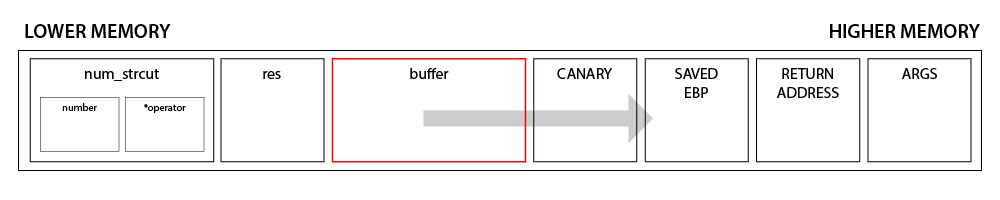
\includegraphics[width=1\columnwidth]{attackStructReel}
	\captionsource{Résultat obtenu de la \og stack frame \fg sur la première attaque}
	{Résultat obtenu de la \og stack frame \fg sur la première attaque}
	{Auteur}
	\label{fig:attackStructReel}
\end{figure}

\subsection{Conclusion}

Cette attaque ne peux pas aboutir et est détectée avec les deux mécanismes de protection. Le but ici est de démontrer les cas de figures où \og \gls{safeStack} \fg permet de se protéger contre des attaques qui ne seraient pas gardée par les \og \gls{stackCookies} \fg, cette attaque est donc abandonée au profit d'une nouvelle approche.


% -----------------------------------------------------------------------------
\section{Bypass du canari}

\subsection{Description théorique de l'attaque}

Le but est toujours d'effectuer une attaque de type \gls{rop}. Pour cela il est
nécessaire d'avoir un point d'entrée afin de démarrer la chaîne de gadgets.
Puisqu'il n'est pas possible de de réécrire les informations sensibles sur la pile
sans passer par le canari, ce second scénario prévoit un moyen de passer outre la
protection en réécrivant correctement ce dernier.

Le scénario est composé de deux phases distinctes. La première consiste à exploiter
une première faille permettant d'aller lire en mémoire la valeur du canari. La
seconde, une fois le canari obtenu, consiste à démarrer la chaîne de gadgets en
réécrivant la valeur de l'adresse de retour de la fonction, en exploitant une deuxième
faille. Ces deux phases doivent être séquentiellement distinctes et dans l'ordre cité.

Pour récupérer la valeur du canari l'argument \texttt{argv[1]} est utilisé comme
format dans une fonction d'affichage. Il est alors possible d'afficher une suite de
valeurs de pointeurs arbitrairement. Une fois le résultat affiché, l'utilisateur est
solicité afin de rentrer une valeur, valeur qui est ensuite stockée dans le tampon via
une méthode vulnérable aux dépassements de tampons.

\begin{figure}[H]
	\centering
	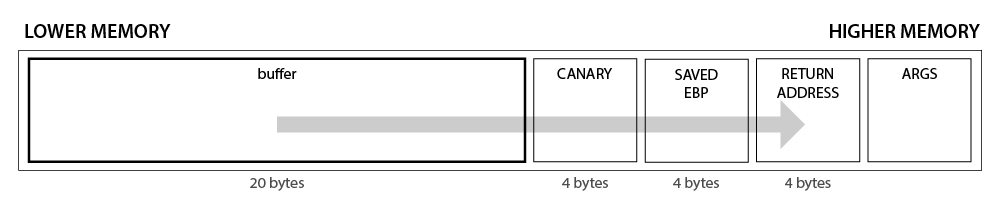
\includegraphics[width=1\columnwidth]{attackCanariLayout}
	\captionsource{Disposition de la pile au sein de la fonction vulnérable}
	{Disposition de la pile au sein de la fonction vulnérable}
	{Auteur}
	\label{fig:attackCanariLayout}
\end{figure}

Le programme imaginé a été conçu de manière à faciliter la mise en place de cette
attaque et ne représente en aucun cas un scénario pertinent au sein d'un environnement
réél. Cependant, les concepts en découlant sont applicables dans tout les cas, ici les
erreurs sont volontairement grossières, mais il est fort probable que des cas
d'attaques similaires, plus complexe à mettre en place, se présentes.

Afin de démontrer la réussite de l'attaque, la chaîne de gadgets doit exécuter deux
fonctions construisant une chaîne de caractères qui est ensuite utilisée comme
paramètre de la fonction \texttt{system()}, au sein d'une troisième fonction. Là
encore, la finalité est prépondérante à la réalité, il faut aussi prendre en compte le
peu de gadgets disponibles au sein d'un programme de si petite taille. La chaîne de
caractères ainsi créée contient la commande \texttt{"echo hacked! > hacked.txt"} afin
de facilement juger la réussite ou l'échec de l'attaque.


\subsection{Implémentation}

La source du programme est plutôt simpliste, la fonction \texttt{main()} appelle la
fonction vulnérable avec l'argument \texttt{argv[1]}. Celui-ci est utilisé directement
comme paramètre de la fonction \texttt{printf()}, un \textit{flush} est ensuite
effectué afin de forcer la sortie dans \textit{stdout}. Le \texttt{buffer} de 20
caractères est initialisé à la ligne 24 et la fonction \texttt{gets()} permet d'écrire
une quantité arbitraire d'octets en mémoire --- ne s'arrête qu'au caractère
\texttt{\textbackslash n} ou \gls{eof} ---, le contenu du tampon est ensuite réaffiché
de manière à simplifier le débogage. Les deux failles de sécurité se trouve donc aux
lignes 25 et 28.

\begin{listing}
	\cfile{02-main/listings/rop2.c}
	\caption{Source du programme lors du second scénario d'attaque}
	\label{lst:rop2}
\end{listing}

Les fonctions \texttt{add\_bin()} et \texttt{add\_sh()} permettent de construire la
chaîne de caractères exécutée dans la fonction \texttt{system()}. Dans la version
originale de l'attaque ces deux fonctions permettaient d'ouvrir un terminal, d'où leur
nom. Afin de représenter au mieux les concepts de \gls{rop}, des paramètres doivent
être passés aux fonctions. Dans ce cas-ci, ces paramètres n'ont pas d'importance.

\subsection{Éxploitation}

La première étape de l'éxploitation consiste à mettre en place un un script permettant
de gérer le \texttt{stdin} et le \texttt{stdout} du programme de manière à récupérer
la valeur du canari et calculer le \textit{payload} à renvoyer.

Le programme avec les \og \gls{stackCookies} \fg est lancé à la ligne 13 du
\autoref{lst:exploit2} avec comme argument $40 \times$ la valeur \texttt{"\%p"}
permettant de faire un \textit{dump} de la mémoire de la pile. La ligne 19 récupère le
\textit{dump} de mémoire puis recherche l'index où apparaît la valeur
\texttt{0x80486ce}. Cette valeur est l'adresse de la fonction \texttt{main()} qui, au
sein de la fonction \texttt{vulnerable\_function()}, équivaut à l'adresse de retour.
En partant de cet index il est ensuite possible de retrouver la valeur du canari.

\begin{listing}
	\pythonfile{02-main/listings/exploit2.py}
	\caption{Script python instrumentant l'attaque ROP du deuxième scénario sur les \og \gls{stackCookies} \fg}
	\label{lst:exploit2}
\end{listing}

Le \textit{payload} doit permettre d'initialiser la pile d'exécution de manière à
chaîner les gadgets. Pour ce faire, le \texttt{buffer} est rempli avec une valeur
arbitraire, dans ce cas \texttt{"A"}, puis on place la valeur du canari, vient ensuite
une valeur quelconque pour remplacer la valeur sauvegardée de \texttt{\%ebp} et enfin
la chaîne de gadgets.

\begin{listing}
	\textfile{02-main/listings/stack.res}
	\caption{État souhaité de la pile d'exécution après injection du \textit{payload}}
	\label{lst:stackAfterPayload}
\end{listing}

Lorsque l'on test la version \og \gls{stackCookies} \fg avec une entrée trop grande,
le dépassement est bien detecté. Le \autoref{lst:stackSmashingDetected} montre le
message qui est affiché avec les diverses informations sur
l'état de la mémoire et de la pile au moment ou l'attaque est détectée.

\begin{listing}
	\textfile{02-main/listings/detected.res}
	\caption{Message obtenu lorsqu'un dépassement de tampon est détecté avec \og \gls{stackCookies} \fg}
	\label{lst:stackSmashingDetected}
\end{listing}

Lorsque l'on exécute le script python le résultat est tout autre. Le canari étant de type
\og \textit{random canary} \fg, finissant toujours par \texttt{\textbackslash x00},
l'éxploitation se déroule sans problème. Le canari est trouvé et réécrit correctement
puis la chaîne de gadgets s'exécute comme prévu. Le script affiche la valeur du canari
trouvé et on constate que le fichier \texttt{hacked.txt} qui n'était pas présent est
bien créé.

\begin{listing}
	\textfile{02-main/listings/powned.res}
	\caption{Message obtenu par le script python du second scénario}
	\label{lst:powned}
\end{listing}

C'est au tour de \og \gls{safeStack} \fg de résister à ce scénario d'attaque.
Pour ce faire, vu qu'il n'y a plus de canari, une adaptation du script
python est faite. Ce script est une version simplifiée du précédent, plus besoin de se
soucier de la première phase.

Lorsqu'on lance l'exécutable compilé avec \og \gls{safeStack} \fg et que l'on rempli
le tampon avec plus de 20 caractères, on remarque que rien ne se passe. Le mécanisme enlève complétement toutes les possibilités d'éxploitations.

\begin{listing}
	\textfile{02-main/listings/attackSafeStack.res}
	\caption{Résultat de l'attaque du second scénario avec \og \gls{safeStack} \fg}
	\label{lst:attackSafeStack}
\end{listing}

Si on regarde de plus prêt l'état de la pile après injection du \textit{payload}, on
constate que celui-ci, n'étant pas présent dans la même région de mémoire, ne peut
plus altérer les pointeurs et les adresses de la pile régulière.

\begin{listing}
	\textfile{02-main/listings/stackSS.res}
	\caption{État de la pile lors du dépassement de tampon avec \og \gls{safeStack} \fg}
	\label{lst:stackSS}
\end{listing}

Les mécansimes de protéction présent au sein des exécutables sont disponibles en \autoref{chap:mecanismeProtection}. La différence des binaires entre les \og \gls{stackCookies} \fg et \og \gls{safeStack} \fg y est présentée.

\begin{listing}
	\pythonfile{02-main/listings/exploit2-ss.py}
	\caption{Script python instrumentant l'attaque ROP du deuxième scénario sur \og \gls{safeStack} \fg}
	\label{lst:exploit2}
\end{listing}

% -----------------------------------------------------------------------------
\section{Conclusions}

\og Safe stack \fg enlève complétement un des biais utilisé afin de dérouté le flot de
contrôle d'une application. Du moment ou tous les tampons sont déplacés hors de portée
des données sensibles de la pile --- adresses de retour, pointeur de fonctions, etc.
--- il est théoriquement impossible de dérouter le flot de contrôle. L'approche
différente de \og \gls{safeStack} \fg par rapport aux \gls{stackCookies} \fg
lui permet de couvrir plus de scénario.
